\documentclass{beamer}
\usepackage[T1]{fontenc}
\usepackage{amsmath}
\usepackage{amssymb}
\usepackage{amsthm}
\usepackage{algorithm}
\usepackage{varwidth}
\usepackage{bm}
\usepackage[noend]{algpseudocode}
\usepackage{xspace}
\usepackage{multirow}
\usepackage{xcolor}
\DeclareRobustCommand{\NAME}{Wideskies\xspace}
\newcommand{\from}{\rightarrow}

\algnewcommand{\algorithmicgiven}{\textbf{given }}
\algnewcommand{\Given}{\algorithmicgiven}

\algnewcommand{\algorithmicselect}{\textbf{select }}
\algnewcommand{\Select}{\algorithmicselect}

\algnewcommand{\algorithmicset}{\textbf{set }}
\algnewcommand{\Set}{\algorithmicset}

\algnewcommand{\algorithmiccompute}{\textbf{compute }}
\algnewcommand{\Compute}{\algorithmiccompute}

\algnewcommand{\algorithmicgoto}{\textbf{go to}}
\algnewcommand{\Goto}[1]{\algorithmicgoto~\ref{#1}}

\newcommand{\Z}{\ensuremath{\mathbf{Z}}}
\newcommand{\zmodn}{\ensuremath{\Z/N\Z}}
\newcommand{\zmodntunits}{\ensuremath{\left(\Z/N^{2}\Z\right)^{\times}}}
\newcommand{\lcm}{\ensuremath{\text{lcm}}}

\mode<presentation> { \usetheme{default} }

\usepackage{graphicx} 
\usepackage{booktabs}
\usepackage{array}
\newcolumntype{L}[1]{>{\raggedright\let\newline\\\arraybackslash\hspace{0pt}}p{#1}}
\newcolumntype{C}[1]{>{\centering\let\newline\\\arraybackslash\hspace{0pt}}p{#1}}
\newcolumntype{R}[1]{>{\raggedleft\let\newline\\\arraybackslash\hspace{0pt}}p{#1}}

\makeatletter
\DeclareRobustCommand*{\&}{%
  \nfss@text{%
    \fontfamily{LinuxBiolinumT-TLF}%
    \selectfont
    \symbol{`\&}%
  }%
}

\usepackage{eso-pic}
\beamertemplatenavigationsymbolsempty
\setbeamertemplate{footline}[frame number]
\newcommand\AtPagemyUpperLeft[1]{\AtPageLowerLeft{%
\put(\LenToUnit{0.9\paperwidth},\LenToUnit{0.9\paperheight}){#1}}}

\AtBeginSection[]{
  \begin{frame}
  \vfill
  \centering
  \begin{beamercolorbox}[sep=8pt,center,shadow=true,rounded=true]{title}
    \usebeamerfont{title}\insertsectionhead\par%
  \end{beamercolorbox}
  \vfill
  \end{frame}
}
\title[Apache Pirk Math
Walkthrough]{
\includegraphics[width=2.5in,keepaspectratio]{ApachePirk_1.png}\\ \bigskip Mathematics $\&$ Algorithms} 

\author{Walter Ray-Dulany} 
\institute[Apache Pirk] 
{
\medskip
\textit{raydulany@apache.org} 
}
% I decided against a date. - Walter
\date{} 

\begin{document}

\begin{frame}
\titlepage 
\end{frame}

\AddToShipoutPictureFG{
  \AtPagemyUpperLeft{{
\includegraphics[width=.5cm,keepaspectratio]{ApachePirkCircle.png}}}
}

\section{Introduction} 

\begin{frame}
\frametitle{Pirk's Wideskies Algorithm}
  Pirk uses the Wideskies algorithm to accomplish scalable PIR.\\~\\
  This algorithm can be broken down into two distinct conceptual pieces:
    \begin{itemize}
      \item Paillier Encryption
      \item The Query-Response-Result algorithms
    \end{itemize}
    ~\\ Before we begin those however, we take a (happily brief) diversion into
    the language of the mathematics involved in this deck.
\end{frame}


\section{Language Preliminaries}
\begin{frame}
  \frametitle{Language Preliminaries}
  The Paillier scheme employs a small amount of group theoretic notation. Let's
  go over that notation briefly.
\end{frame}

\begin{frame}
  \frametitle{Language Preliminaries}
  \begin{itemize}
    \item \zmodn: This is the group of integers modulo $N$; it can be thought of
      as all numbers $0\leq k < N$, with modular addition (e.g.\ for $N=5$,
      $1+7 \equiv 3\mod N$).\\~\\ This is a group under addition.\\~\\
    \item $(\zmodn)^\times$: This is the multiplicative group of integers modulo
      $N$, also called the units of $\zmodn$. Sometimes denoted
      $(\mathbf{Z}/N\mathbf{Z})^*$, this is the set of $0\leq k < N$ that are
      relatively prime to $N$ (that is, $k$ and $N$ share no factors, or
      equivalently the greatest common denominator ($\gcd$) of $k$ and $N$ is $1$). One
      can also think of this as the set of $k\in\zmodn$ such that there exists
      a $k^{-1}\in\zmodn$ with $k\cdot k^{-1} \equiv 1\mod N$.\\~\\
      This is a group under multiplication.
  \end{itemize}
\end{frame}

\begin{frame}
  \frametitle{Language Preliminaries}
Using the above notation, we can see that 
\begin{equation*}
  \zmodntunits = \{0\leq k<N^2: \gcd(k,N^2) = 1\}.
\end{equation*}~\\
If $N$ happens to be an RSA modulus,
$N=pq$, $p$ and $q$ primes, then $\zmodntunits$ is just all numbers between $0$
(inclusive) and $N^2$ (exclusive) that are not divisible by either $p$ or
$q$.
\end{frame}

\begin{frame}
  \frametitle{Language Preliminaries}
  \begin{itemize}
    \item Order In \zmodn: The order of an element $k\in\zmodn$ is the least integer $e$
      such that $e\cdot k = 0\mod N$.
    \item Order in \zmodntunits: The order of an element $a\in\zmodntunits$ is
      the least integer $e$ such that $a^e = 1\mod N^2$.
  \end{itemize}
  In both cases, order is well defined (i.e.\ it exists and makes sense) for
  all elements of the groups.
\end{frame}

\begin{frame}
  \frametitle{Language Preliminaries}
  For a more in depth discussion of these, and closely related, terms, please
  see 
  \mbox{\scriptsize \url{http://www.math.nagoya-u.ac.jp/~richard/teaching/s2015/Group_2.pdf}}
\end{frame}

\section{Paillier Encryption}
\begin{frame}
\frametitle{Paillier Encryption}
Paillier encryption is a partially homomorphic public key scheme that relies on
the function $$\mathcal{E}_g:\zmodn\times(\zmodn)^\times\rightarrow
\zmodntunits$$ given by $$\mathcal{E}_g(x,y) = g^x y^N \mod N^2,$$
$g\in\zmodntunits$. Here, $\zmodn$ is the plaintext space and $\zmodntunits$ is
the ciphertext space.\\~\\
When the order of $g$ is a non-zero multiple of $N$, $\mathcal{E}_g$ is a bijection.
\end{frame}

\begin{frame}
  \frametitle{Paillier Prerequisites}
\begin{itemize}
  \item Public key: $(N,g)$, $N$ an RSA modulus $N=pq$, $p$ and $q$ primes of
    approximately the same bit-length, and $g\in \zmodntunits$ such that the
    order of $g$ is a nonzero multiple of $N$. 
  \item Private key: $\lambda(N)$, where $\lambda$ is the Carmichael function
    \begin{align*}
      \lambda(N) &= \lcm(p-1,q-1)
    \end{align*}
  that gives the exponent of $(\zmodn)^\times$.
  \item Plaintext space: \zmodn.
  \item Ciphertext space: \zmodntunits.
\end{itemize}
~\\
{\footnotesize We can also consider the pair $(p,q)$ to be the private key, as $\lambda(N)$ is
quickly and easily derived from it. Note that $\lambda(N)$ is coprime to $N$.}
\end{frame}

\begin{frame}
  \frametitle{What Do We Mean By `Homomorphic Encryption'?}
  An encryption scheme is fully homomorphic if it is a homomorphism from
  plaintext space to ciphertext space for arbitrary operations and arbitrary
  numbers of such operations. If this definition seems squishy and not very
  mathematical, that's because it is; it's hard to find a proper mathematical
  definition of this term.\\~\\

  An encryption scheme is partially homomorphic if it is a homomorphism for
  only some operations, or for only a few consecutive operations.\\~\\
\end{frame}

\begin{frame}
  \frametitle{Paillier Encryption is Homomorphic}
  Paillier encryption is a partial homomorphism between addition in \zmodn\ and
  multiplication in \zmodntunits.\\~\\

  Denote Paillier encryption by $\mathcal{E}_g$ and decryption by $\mathcal{D}_g$,
  and let $m$ and $m'\in \zmodn$. Then 
    \begin{align*}
        D(\mathcal{E}(m) \mathcal{E}(m') \bmod N^2) &= (m + m') \bmod N \\
        D(\mathcal{E}(m)^k \bmod N^2) &= km \bmod N, \, k \in \mathbf{N}
    \end{align*}
    ~\\
    Note that the second equality follows immediately from the first.
\end{frame}

\section{General Paillier Algorithm}

\begin{frame}
\frametitle{Paillier Supporting Function}
Let $X=\{u<N^2 : u = 1 \mod N\}$ and let $L:X\rightarrow \zmodn$ be
defined by 
\begin{equation*}L(u) = \frac{u-1}{N} \mod N.\end{equation*}
This function is well defined over \zmodntunits.
\end{frame}

\begin{frame}
\frametitle{General Paillier Encryption}
The general Paillier algorithm differs only slightly from Pirk's version.
\begin{algorithm}[H]
  \caption{General Paillier encryption and decryption.}\label{alg.paillier_encrypt_original}
  \begin{algorithmic}[1]
    \Procedure{Paillier encryption}{}
    \State \begin{varwidth}[t]{\linewidth}
      \Given \(N\), a random \(g \in \zmodntunits\) of order a nonzero\par
  multiple of $N$, and a message \(m\in\zmodn\)
      \end{varwidth}
    \State \Select a random value \(\zeta\in \left(\zmodn\right)^{\times}\)
    \State \Return \(\mathcal{E}(m) = g^m \zeta^{N}\bmod{N^{2}}\)
    \EndProcedure
  \end{algorithmic}
  \begin{algorithmic}[1]
    \Procedure{Paillier decryption}{}
    \State \Given \(N\), \(\lambda(N)\), \(g\), and ciphertext \(c \in \zmodntunits\)
    \State \Return m = \(\frac{L( c^{\lambda(N)}\bmod N^{2})}{L( g^{\lambda(N)}\bmod N^{2})}\bmod N\)
    \EndProcedure
  \end{algorithmic}
\end{algorithm}
\end{frame}

\begin{frame}
\frametitle{Paillier Works}
  It is a straightforward exercise to check that 
  \begin{itemize}
    \item $D(\mathcal{E}(m)) = m$
    \item $D(\mathcal{E}(m)\mathcal{E}(m')\bmod N^2) = (m + m') \bmod N $
  \end{itemize}
\end{frame}

\section{Paillier As Used In \NAME}
\begin{frame}
\frametitle{Paillier As Used In \NAME}
The version of Paillier used in \NAME is a computationally simpler variant of the
full Paillier scheme that sacrifices no security over the general case.
\end{frame}

\begin{frame}
  \frametitle{Converting Between The Two}
  Pirk's simplified version of Paillier simply uses
  \begin{align*}
    g &\equiv 1 + N \mod N^2\\
    \implies L(g^{\lambda(N)} \mod N^2) &= \lambda(N),
  \end{align*}
  the proof of which is a straightforward exercise.
\end{frame}

\begin{frame}
\frametitle{Paillier As Used In \NAME}
\begin{algorithm}[H]
  \caption{Paillier encryption and decryption}\label{alg.paillier_encrypt}
  \begin{algorithmic}[1]
    \Procedure{Paillier encryption}{}
    \State \Given \(N\) and a message \(m\in\zmodn\)
    \State \Select a random value \(\zeta\in\zmodntunits\)
    \State \Return \(\mathcal{E}(m) = (1+mN)\zeta^{N}\bmod{N^{2}}\)
    \EndProcedure
  \end{algorithmic}

  \begin{algorithmic}[1]
    \Procedure{Paillier decryption}{}
    \State \Given \(N\), \(\lambda(N)\), and a ciphertext \(c\in\zmodntunits\)
    \State \Set \(\mu = \lambda(N)^{-1}\bmod N\)
    \Comment Recall \(\gcd(\lambda(N), N) = 1\)
    \State \Set \(\hat{c} = c^{\lambda(N)}\bmod N^{2}\)
    \State\label{step.div}\Set \(\hat{m} = L(c^{\lambda(N)}\bmod N^{2})\)
    \State \Return \(\hat{m}\mu\bmod N\)
    \EndProcedure
  \end{algorithmic}
\end{algorithm}
\end{frame}

\begin{frame}
  \frametitle{Paillier Reference}
  For more on Paillier encryption and the (hypothesized) hard problem upon
  which it is based, see\\~\\
  \mbox{\scriptsize \url{https://pirk.incubator.apache.org/papers/1999_asiacrypt_paillier_paper.pdf}}\\~\\
  on Pirk's website.
\end{frame}

\section{Wideskies}

\begin{frame}
  \frametitle{Wideskies Parameters}
  The algorithm requires the following parameters, which are not independent
  (see the next slide).
  \begin{itemize}
    \item $N$, the Paillier modulus
    \item $B$, the bit-length of $N$
    \item $H$ (or $H_k$), a keyed hash function (with key k)
    \item $\ell$, the bit length of the output of $H$, i.e.\
      $H_k:\mathbf{Z}\rightarrow (\mathbf{Z}/2\mathbf{Z})^\ell$
    \item $\tau$, the number of search terms
    \item $\delta$, the number of bits of data returned for each search hit
    \item $b$ the chunk size, in bits, determining how data is split among
      responses.
    \item $r$, the number of responses that can be returned per query request
      period per search term
  \end{itemize}
\end{frame}

\begin{frame}
  \frametitle{Parameter Relationships}
  \begin{itemize}
    \item $2^{b\tau} < N$: there must be space in the modulus to hold all the
      data, even if each search term hits as often as possible.
    \item $\tau < 2^\ell$: Although the paper permits search term hash
    collisions, Pirk does not permit them. Typically $\tau \ll 2^\ell$
    \item $b|\delta$: Chunk size must evenly divide the data size
    \item $\frac{\delta}{b} | r$: the number of chunks per returned datum must
      divide the number of responses, for bandwidth efficiency.
    \item $H$: Must be pseudo-random but need not be cryptographically secure.
  \end{itemize}
\end{frame}

\begin{frame}
  \frametitle{Public Parameters}
  All of \begin{equation*}H, \ell, N, B, \delta, b, \text{and } r\end{equation*}
  are public, that is, must be shared between the client and server.\\~\\

  Note that the fact that $2^{b\tau} < N$ gives some information on the number
  of search terms the client is using; the amount of this information can be
  decreased without bound by choosing $N$ and $\ell$ to be much larger than
  would be otherwise necessary; this necessarily causes a performance hit.
\end{frame}

\section{Wideskies Algorithm, Without Encryption}
\begin{frame}
  \frametitle{Wideskies Without Encryption?}
  The Wideskies algorithm is of sufficient complexity that it can be useful to
  go through the algorithm without the encryption and decryption steps first,
  in order to orient ourselves.\\~\\
  After, it will be straightforward to see the
  changes that using the Paillier encryption requires.
\end{frame}

\section{Query, Without Encryption}
\begin{frame}
  \frametitle{The Query Algorithm, Without Encryption}
  Let $T_0,\ldots,T_{\tau-1}\in\zmodn$ be our search terms.
  \begin{algorithm}[H]
  \caption{Query Formation Algorithm version
    1}\label{alg.plain_form_1}
\begin{algorithmic}[1]
  \State\label{step.key}Choose a random key \(k\) for \(H\).
  \State Compute \(H_{k}(T_{0}),\ldots,H_{k}(T_{\tau-1})\).
  \While{\(\mathrm{card}\left(\{H_{k}(T_{0}),\ldots,H_{k}(T_{\tau-1})\}\right)
    < \tau\)}
  \State \Goto{step.key}
  \Comment If there are hash collisions, pick a new key.
  \EndWhile
  \For{\(i=0,\ldots,2^{\ell}-1\)}
  \State\label{step.set}Set \begin{equation*}
    E_{i} = \left\{\begin{array}{l l} 
    2^{jb} & \mbox{ if } i = H_{k}(T_{j}); \\
    0 & \mbox{otherwise.}
    \end{array}
    \right.
  \end{equation*}
  \EndFor
  \State\Return \(\{E_{0},\ldots,E_{2^{\ell}-1}, H, k, N\}\)
\end{algorithmic}
\end{algorithm}
\end{frame}

\begin{frame}
  \frametitle{Query Notes, Without Encryption}
  Since $\tau \ll 2^\ell$, we expect most of the $E_i$ to be zero.\\~\\
  We will typically denote $H_k(T)$ by $\mathcal{T}$ and its associated $E$ by
  $E_\mathcal{T}$. If we wish to keep track of a specific $T$ we will write
  $\mathcal{T}_j$ and $E_{\mathcal{T}_j}$.
\end{frame}

\section{Response, Without Encryption}
\begin{frame}
  \frametitle{Response Initialization, Without Encryption}
  We must initialize some values before forming the response.
  \begin{enumerate}
    \item $c_0,\ldots,c_{2^\ell - 1} = 0$, counters to keep track of the number
      of times each $E_\mathcal{T}$ has been seen.
    \item $Y_0,\ldots,Y_{r-1} = 0$, response vectors.
  \end{enumerate}
\end{frame}

\begin{frame}
  \frametitle{Response Data, Without Encryption}
  Responder information comes in pairs $(T, D)$ where $T$ is a (potential)
  search term, and $D$ is $T$'s associated response datum, which will be
  returned if $T$ is a search term.\\~\\

  We view $D$ as a $\delta$-long bit stream $(d_0,\ldots,d_{\delta-1})$, and
  break $D$ up into $\delta/b$ chunks $D_i$ as 
  \begin{equation*}
    D_i = (d_{i\cdot b}, d_{i\cdot b+1},\ldots,d_{(i+1)\cdot b-1}),\ i=0,\ldots,\delta/b-1.
  \end{equation*}\\~\\
  For example, if $D=011010$ and $b=3$, then
  \begin{align*}
    D_0 &= 011\\
    D_1 &= 010
  \end{align*}
\end{frame}

\begin{frame}
  \frametitle{Response Algorithm, Without Encryption}
  \begin{algorithm}[H]
  \caption{Stream processing, plaintext version}\label{alg.plain_stream}
\begin{algorithmic}[1]
\State \textbf{Input}:  $\mathbf{T} = \{ (T,D) \}$
\For{$(T,D) \in \mathbf{T}$}
  \State Compute \(\mathcal{T} = H_{k}(T)\)
  \If{\(c_{\mathcal{T}} + \frac{\delta}{b} > r\)}\label{step.if}
  \Comment The space allocated for term \(T\) is full.
  \State \Return \label{step.return}
\Else
  \State Split \(D\) into \(b\)-bit chunks
  \(D_{0},\ldots,D_{(\delta/b)-1}\).
  \For{\(i=0,\ldots,(\delta/b)-1\)}
  \State\label{step.multiply}Set \(\mathcal{D}_{i} = D_{i}E_{\mathcal{T}}\bmod N\)
  \Comment Nonzero only if \(E_{\mathcal{T}}\neq 0\).
  \State Set \(Y_{i+c_{\mathcal{T}}} =
  Y_{i+c_{\mathcal{T}}}+\mathcal{D}_{i}\bmod N\)
  \EndFor
  \State Set \(c_{\mathcal{T}} = c_{\mathcal{T}}+(\delta/b)\)
\EndIf

\EndFor
\State{\textbf{Output}}: \(Y_{0},\ldots,Y_{r-1}\)
\end{algorithmic}
\end{algorithm}
\end{frame}

\begin{frame}
  \frametitle{Response Example, Without Encryption}
  Let's look at how the response would look on the first four $(T,D)$ pairs that
  pass through the algorithm.
\end{frame}

\begin{frame}
  \frametitle{Response Example Setup, Without Encryption}
  Suppose that among our search terms are $T$ and $T'$, with 
  \begin{align*}
    H_k(T) &= j\text{ and}\\
    H_k(T') &= j'.
  \end{align*}~\\

  
  Suppose that $T''$, with $H_k(T'')=j''$, is \emph{not} a search term.\\~\\

  Let the responder see, in order, the pairs $(T, D^0)$, $(T', D^1)$,
  $(T'', D^2)$, $(T, D^3)$.\\~\\

  The $Y_i$ are formed by summing down the columns in following matrices.
\end{frame}

\begin{frame}
  \frametitle{Response Example Start, Without Encryption}
  No terms have yet been evaluated.
  \begin{center}
  \begin{tabular}{c  C{1.55cm}  c  C{1.55cm}  C{1.55cm}  c  C{1.55cm}  }
   {\scriptsize Index}             & $Y_0$\qquad            & $\cdots$\qquad         & $Y_{\delta/b-1}$\qquad & $Y_{\delta/b}$\qquad   & $\cdots$\qquad         & $Y_{2\delta/b-1}$\qquad\\\toprule
    $\vdots$ & \multicolumn{6}{l}{$\qquad$}\\
 {\footnotesize$j$} & 0                        & $\cdots$                         & 0                         & 0                         & $\cdots$                         & 0                         \\
    $\vdots$ & \multicolumn{6}{l}{$\qquad$}\\
 {\footnotesize$j'$}  & 0                      & $\cdots$                           & 0                           & 0                      & $\cdots$                           & 0\\
    $\vdots$ & \multicolumn{6}{l}{$\qquad$}\\
     {\footnotesize$j''$}  & 0 & $\cdots$                           & 0         & 0                      & $\cdots$                           & 0\\
    $\vdots$ & \multicolumn{6}{l}{$\qquad$}\\\bottomrule
  \end{tabular}
  \end{center}
  $c_{j} = 0$, $c_{j'} = 0$, $c_{j''} = 0$.
\end{frame}

\begin{frame}
  \frametitle{Response Example: First Term, Without Encryption}
  $(T, D^0)$ enters and is proccessed; hit:
  \begin{center}
  \begin{tabular}{c  C{1.55cm}  c  C{1.55cm}  C{1.55cm}  c  C{1.55cm}  }
     {\scriptsize Index}             & $Y_0$\qquad            & $\cdots$\qquad         & $Y_{\delta/b-1}$\qquad & $Y_{\delta/b}$\qquad   & $\cdots$\qquad         & $Y_{2\delta/b-1}$\qquad\\\toprule
     $\vdots$ & \multicolumn{6}{l}{$\qquad$}\\
     {\footnotesize$j$} & {\footnotesize $\bm{D^0_0} 2^{jb}$}                         & $\cdots$                         & {\footnotesize $\bm{D^0_{\delta/b-1}} 2^{jb}$}                      & 0                         & $\cdots$                         & 0                         \\
     $\vdots$ & \multicolumn{6}{l}{$\qquad$}\\
     {\footnotesize$j'$}  & 0 & $\cdots$                           & 0                           & 0                      & $\cdots$                           & 0\\
     $\vdots$ & \multicolumn{6}{l}{$\qquad$}\\
     {\footnotesize$j''$}  & 0 & $\cdots$                           & 0         & 0                      & $\cdots$                           & 0\\
    $\vdots$ & \multicolumn{6}{l}{$\qquad$}\\\bottomrule
  \end{tabular}
  \end{center}
  $\bm{c_{j} = \delta/b}$, $c_{j'} = 0$, $c_{j''} = 0$.
\end{frame}

\begin{frame}
  \frametitle{Response Example Second Term, Without Encryption}
  $(T', D^1)$ enters and is proccessed; hit:
  \begin{center}
  \begin{tabular}{c  C{1.55cm}  c  C{1.55cm}  C{1.55cm}  c  C{1.55cm}  }
     {\scriptsize Index}             & $Y_0$\qquad            & $\cdots$\qquad         & $Y_{\delta/b-1}$\qquad & $Y_{\delta/b}$\qquad   & $\cdots$\qquad         & $Y_{2\delta/b-1}$\qquad\\\toprule
     $\vdots$ & \multicolumn{6}{l}{$\qquad$}\\
     {\footnotesize$j$} & {\footnotesize ${D^0_0} 2^{jb}$}                         & $\cdots$                         & {\footnotesize ${D^0_{\delta/b-1}} 2^{jb}$}                      & 0                         & $\cdots$                         & 0                         \\
     $\vdots$ & \multicolumn{6}{l}{$\qquad$}\\
     {\footnotesize$j'$}  & {\footnotesize $\bm{D^1_0} 2^{j'b}$} & $\cdots$                           & {\footnotesize $\bm{D^1_{\delta/b-1}} 2^{j'b}$}                           & 0                      & $\cdots$                           & 0\\
     $\vdots$ & \multicolumn{6}{l}{$\qquad$}\\
     {\footnotesize$j''$}  & 0 & $\cdots$                           & 0         & 0                      & $\cdots$                           & 0\\
    $\vdots$ & \multicolumn{6}{l}{$\qquad$}\\\bottomrule
  \end{tabular}
  \end{center}
  $c_{j} = \delta/b$, $\bm{c_{j'} = \delta/b}$, $c_{j''} = 0$.
\end{frame}

\begin{frame}
  \frametitle{Response Example Third Term, Without Encryption}
  $(T'', D^2)$ enters and is proccessed; no hit:
  \begin{center}
  \begin{tabular}{c  C{1.55cm}  c  C{1.55cm}  C{1.55cm}  c  C{1.55cm}  }
     {\scriptsize Index}             & $Y_0$\qquad            & $\cdots$\qquad         & $Y_{\delta/b-1}$\qquad & $Y_{\delta/b}$\qquad   & $\cdots$\qquad         & $Y_{2\delta/b-1}$\qquad\\\toprule
     $\vdots$ & \multicolumn{6}{l}{$\qquad$}\\
     {\footnotesize$j$} & {\footnotesize ${D^0_0} 2^{jb}$}                         & $\cdots$                         & {\footnotesize ${D^0_{\delta/b-1}} 2^{jb}$}                      & 0                         & $\cdots$                         & 0                         \\
     $\vdots$ & \multicolumn{6}{l}{$\qquad$}\\
     {\footnotesize$j'$}  & {\footnotesize ${D^1_0} 2^{j'b}$} & $\cdots$                           & {\footnotesize ${D^1_{\delta/b-1}} 2^{j'b}$}                           & 0                      & $\cdots$                           & 0\\
     $\vdots$ & \multicolumn{6}{l}{$\qquad$}\\
     {\footnotesize$j''$}  & {\footnotesize $\bm{D^2_0} \cdot 0$}  & $\cdots$                           & {\footnotesize $\bm{D^2_{\delta/b-1}} \cdot 0$}     & 0                      & $\cdots$                           & 0\\
    $\vdots$ & \multicolumn{6}{l}{$\qquad$}\\\bottomrule
  \end{tabular}
  \end{center}
$c_{j} = \delta/b$, $c_{j'} = \delta/b$, $\bm{c_{j''} = \delta/b}$.
\end{frame}

\begin{frame}
  \frametitle{Response Example Fourth Term, Without Encryption}
  $(T, D^3)$ enters and is proccessed; hit:
  \begin{center}
  \begin{tabular}{c  C{1.55cm}  c  C{1.55cm}  C{1.55cm}  c  C{1.55cm}  }
     {\scriptsize Index}             & $Y_0$\qquad            & $\cdots$\qquad         & $Y_{\delta/b-1}$\qquad & $Y_{\delta/b}$\qquad   & $\cdots$\qquad         & $Y_{2\delta/b-1}$\qquad\\\toprule
     $\vdots$ & \multicolumn{6}{l}{$\qquad$}\\
     {\footnotesize$j$} & {\footnotesize ${D^0_0} 2^{jb}$}                         & $\cdots$ & {\footnotesize ${D^0_{\delta/b-1}} 2^{jb}$}                      & {\footnotesize $\bm{D^3_0} 2^{jb}$}                         & $\cdots$ & {\footnotesize $\bm{D^3_{\delta/b-1}} 2^{jb}$}                         \\
     $\vdots$ & \multicolumn{6}{l}{$\qquad$}\\
     {\footnotesize$j'$}  & {\footnotesize ${D^1_0} 2^{j'b}$} & $\cdots$                           & {\footnotesize ${D^1_{\delta/b-1}} 2^{j'b}$}                           & 0                      & $\cdots$                           & 0\\
     $\vdots$ & \multicolumn{6}{l}{$\qquad$}\\
     {\footnotesize$j''$}  & {\footnotesize $\bm{D^2_0} \cdot 0$}  & $\cdots$                           & {\footnotesize $\bm{D^2_{\delta/b-1}} \cdot 0$}     & 0                      & $\cdots$                           & 0\\
    $\vdots$ & \multicolumn{6}{l}{$\qquad$}\\\bottomrule
  \end{tabular}
  \end{center}
  $\bm{c_{j} = 2\delta/b}$, $c_{j'} = \delta/b$, $c_{j''} = \delta/b$.
\end{frame}

\section{Result, Without Encryption}
\begin{frame}
  \frametitle{Result, Without Encryption}
  The algorithm for getting the results out of the response return is
  straightforward. To begin,\\~\\
  \begin{itemize}
    \item Write $Y_i = \sum_{k=0}^{\tau - 1} 2^{kb}P_{ki}$ in base $2^b$, where
      $P_{ki}$ is the value of the $k^{\text{th}}$ row in the
      $i^{\text{th}}$ column. Note each $P_{ki}$ is $b$-bits long, and therefore
      $Y_i < N$.
    \item $Y_i$ will have data on search term $T$ if and only if $T$ was
      seen $i+1$ times before the responder returned.
  \end{itemize}
\end{frame}

\begin{frame}
  \frametitle{Result Algorithm, Without Encryption}
  \begin{algorithm}[H]

  \caption{Data recovery, plaintext version}\label{alg.plain_recover}
\begin{algorithmic}[1]
  \State Set \(M = 2^{j b}(2^{b}-1)\)
  \Comment $b$ $1$s left-shifted $jb$ places.
  \For{\(\eta=1,\ldots,(rb/\delta)\)}
  \Comment At most \(rb/\delta\) hits can be returned.
  \For{\(i=0,\ldots,(\delta/b)-1\)}
  \Comment Each hit uses \(\delta/b\) chunks.
  \State\label{step.mask}Set \(D_{i} = Y_{(\eta-1)(\delta/b)+i}\&M\)
  \Comment ``\(\&\)'' denotes bit-wise \texttt{AND}.
  \State\label{step.shift}Set \(D_{i} = D_{i}/2^{jb}\)
  \Comment Step \ref{step.mask} ensures \(2^{jb}\mid D_{i}\)
  \EndFor
  \State Set \(X_{\eta} = D_{0}\|D_{1}\|\ldots\|D_{(\delta/b)-1}\)
  \EndFor
  \State \Return \(X_{1},\ldots,X_{(rb/\delta)}\)
  \Comment the data corresponding to selector \(T_{j}\)
\end{algorithmic}
\end{algorithm}
\end{frame}

\section{Wideskies Algorithm, With Encryption}
\begin{frame}
  \frametitle{Adding Encryption To The Mix}
  Adding encryption is straightforward. The following slides have the
  encryption-enabled algorithms, with the differences from the earlier slides
  in bold.
\end{frame}

\section{Query, Encrypted}
\begin{frame}
  \frametitle{Query, Encrypted}
  \begin{algorithm}[H]
  \caption{Query formation, ciphertext version 1}\label{alg.cipher_form_1}
\begin{algorithmic}[1]
  \State\label{step.key_2}Choose a random key \(k\) for \(H\).
  \State Compute \(H_{k}(T_{0}),\ldots,H_{k}(T_{\tau-1})\).
  \While{\(\mathrm{card}\left(\{H_{k}(T_{0}),\ldots,H_{k}(T_{\tau-1})\}\right)
    < \tau\)}
  \State \Goto{step.key_2}
  \EndWhile
  \For{\(i=0,\ldots,2^{\ell}-1\)}
  \State Set
  {
  \bfseries\boldmath
  \begin{equation*}
    \mathcal{E}_{i} = \left\{\begin{array}{l l}
        \mathcal{E}(2^{jb}) & \mbox{ if }i=H_{k}(T_{j})\mbox{ for some
        }j\in\{0,\ldots,\tau-1\} \\
        \mathcal{E}(0) & \mbox{ otherwise.}
      \end{array}
    \right.
  \end{equation*}}
  \EndFor
  \State \Return \(\{\mathcal{E}_{0},\ldots,\mathcal{E}_{2^{\ell}-1}, H,
  k, N\}\)
\end{algorithmic}
\end{algorithm}
\end{frame}

\section{Response, Encrypted}
\begin{frame}
  \frametitle{Response Initialization, Encrypted}
  As before, we must initialize some values before forming the response.
  \begin{enumerate}
    \item $c_0,\ldots,c_{2^\ell - 1} = 0$, counters to keep track of the number
      of times each {\boldmath $\mathcal{E}_\mathcal{T}$} has been seen.
    \item {\bfseries\boldmath $Y_0,\ldots,Y_{r-1} = 1$, response vectors.}
  \end{enumerate}
\end{frame}

\begin{frame}
  \frametitle{Response, Encrypted}
  \begin{algorithm}[H]
  \caption{Stream processing, ciphertext version}\label{alg.cipher_processing}
\begin{algorithmic}[1]
\State \textbf{Input}:  $\mathbf{T} = \{ (T,D) \}$
\State \textbf{Initialize:}
\State \qquad Counters $c_i = 0 \, , \, 0 \leq i \leq (2^l -1)$
\State \qquad Paillier ciphertext values  $\mathcal{Y}_{j} = 1 \, , \, 0 \leq j \leq (r-1)$
\For{$(T,D) \in \mathbf{T}$}
  \State Compute \(\mathcal{T} = H_{k}(T)\)
  \If{\(c_{\mathcal{T}}+\frac{\delta}{b} > r\)}
  \State \Return
  \Else
  \State Split \(D\) into \(b\)-bit chunks,
  \(D=D_{0},\ldots,D_{(\delta/b)-1}\) \label{step.datachunk}
  \For{\(i=0,\ldots,(\delta/b)-1\)}
  \State {\bfseries\boldmath Set \(\mathcal{D}_{i} =
  \mathcal{E}_{\mathcal{T}}^{D_{i}}\bmod N^{2}\)}
  \State {\bfseries\boldmath Set \(\mathcal{Y}_{i+c_{\mathcal{T}}} =
  \mathcal{Y}_{i+c_{\mathcal{T}}}\mathcal{D}_{i}\bmod N^{2}\)}
  \EndFor
  \State Set \(c_{\mathcal{T}} = c_{\mathcal{T}}+(\delta/b)\)
  \EndIf
\EndFor
\State{\textbf{Output}}: \(\mathcal{Y}_{0},\ldots,\mathcal{Y}_{r-1}\)
\end{algorithmic}
\end{algorithm}
\end{frame}

\section{Result, Encrypted}
\begin{frame}
  \frametitle{Result, Encrypted (and then Decrypted)}
  Actually literally the same algorithm as before is used; the only difference
  is that we first decrypt the encrypted $\mathcal{Y}_i$.
\end{frame}

\section{Distributed Version}
\begin{frame}
  \frametitle{Distributed Version}
  The paper goes over how to do the distributed version; the change is
  straightforward, and our earlier example slides make it easy to see how it
  works.
\end{frame}

\begin{frame}
  \frametitle{Distributed Difference:\\ Unencrypted Sums, Encrypted Products}
  Recall our example matrix:
  \begin{center}
  \begin{tabular}{c  C{1.55cm}  c  C{1.55cm}  C{1.55cm}  c  C{1.55cm}  }
     {\scriptsize Index}             & $Y_0$\qquad            & $\cdots$\qquad         & $Y_{\delta/b-1}$\qquad & $Y_{\delta/b}$\qquad   & $\cdots$\qquad         & $Y_{2\delta/b-1}$\qquad\\\toprule
     $\vdots$ & \multicolumn{6}{l}{$\qquad$}\\
     {\footnotesize$j$} & {\footnotesize ${D^0_0} 2^{jb}$}                         & $\cdots$ & {\footnotesize ${D^0_{\delta/b-1}} 2^{jb}$}                      & {\footnotesize ${D^3_0} 2^{jb}$}                         & $\cdots$ & {\footnotesize ${D^3_{\delta/b-1}} 2^{jb}$}                         \\
     $\vdots$ & \multicolumn{6}{l}{$\qquad$}\\
     {\footnotesize$j'$}  & {\footnotesize ${D^1_0} 2^{j'b}$} & $\cdots$                           & {\footnotesize ${D^1_{\delta/b-1}} 2^{j'b}$}                           & 0                      & $\cdots$                           & 0\\
     $\vdots$ & \multicolumn{6}{l}{$\qquad$}\\
     {\footnotesize$j''$}  & {\footnotesize $\bm{D^2_0} \cdot 0$}  & $\cdots$                           & {\footnotesize $\bm{D^2_{\delta/b-1}} \cdot 0$}     & 0                      & $\cdots$                           & 0\\
     $\vdots$ & \multicolumn{6}{l}{$\qquad$}\\\bottomrule
  \end{tabular}
  \end{center}
\end{frame}

\begin{frame}
  \frametitle{Distributed Difference:\\ Unencrypted Sums, Encrypted Products}
  When we moved to an encrypted algorithm, all of the $D_i$-long sums of
  $E_i$ became
  $\mathcal{E}_i^{\mathcal{D}_i}$.\\~\\
  In the distributed version, we actually make matrix components rather than
  the fake matrix of $D_i$ in certain bit-positions we had earlier.\\~\\
  
  In the matrix, rows are indexed by $0 \leq \mathcal{T} \leq 2^\ell
  -1$, columns by $0 \leq j \leq r-1$.
\end{frame}


\begin{frame}
  \frametitle{Distributed Difference:\\ Unencrypted Sums, Encrypted Products}
  As before, let 
  \begin{align*}
    H_k(T) &= j,\\
    H_k(T') &= j',\text{ and}\\
    H_k(T'') &= j'',
  \end{align*}
  with $T$ and $T'$ search terms and $T''$ not.\\~\\
  Notice that this time we won't simply discard the data $D_2$ from $T''$;
  we no longer multiply it by zero, but use it as the exponent of
  $\mathcal{E}_{j''}$, which is an encryption of $0$.
\end{frame}

\begin{frame}
  \frametitle{Distributed Difference:\\ Unencrypted Sums, Encrypted Products}
  The matrix in the encrypted setting:
  \begin{center}
  \begin{tabular}{c  C{1.35cm}  c  C{1.35cm}  C{1.35cm}  c  C{1.35cm}  }
     {\scriptsize Index}             & $\mathcal{Y}_0$\qquad            & $\cdots$\qquad         & $\mathcal{Y}_{\delta/b-1}$\qquad & $\mathcal{Y}_{\delta/b}$\qquad   & $\cdots$\qquad         & $\mathcal{Y}_{2\delta/b-1}$\qquad\\\toprule
     $\vdots$ & \multicolumn{6}{l}{$\qquad$}\\
     {\footnotesize$j$} & {\footnotesize $\mathcal{E}_j^{D^0_0}$} & $\cdots$ & {\footnotesize $\mathcal{E}_j^{D^0_{\delta/b-1}}$}                      & {\footnotesize $\mathcal{E}_j^{D^3_0}$}                         & $\cdots$ & {\footnotesize $\mathcal{E}_j^{D^3_{\delta/b-1}}$}                         \\
     $\vdots$ & \multicolumn{6}{l}{$\qquad$}\\
     {\footnotesize$j'$}  & {\footnotesize $\mathcal{E}_{j'}^{D^1_0}$} & $\cdots$                           & {\footnotesize $\mathcal{E}_{j'}^{D^1_{\delta/b-1}}$}                           & 1                      & $\cdots$                           & 1\\
     $\vdots$ & \multicolumn{6}{l}{$\qquad$}\\
     {\footnotesize$j''$}  & {\footnotesize $\mathcal{E}_{j''}^{D^2_0}$} & $\cdots$                           & {\footnotesize $\mathcal{E}_{j''}^{D^2_{\delta/b-1}}$}                           & 1                      & $\cdots$                           & 1\\
     $\vdots$ & \multicolumn{6}{l}{$\qquad$}\\\bottomrule
  \end{tabular}
  \end{center}
\end{frame}

\begin{frame}
  \frametitle{Algorithm In Matrix Form}
  \begin{algorithm}[H]
  \caption{Responder -  Matrix Variant}\label{alg.matrix_processing}
\begin{algorithmic}[1]
  \State {\scriptsize \textbf{Input:}  $\mathbf{T} = \{ (T,D) \}$}
\State{\scriptsize  \textbf{Initialize:}}
\State{\scriptsize  \qquad Counters $c_i = 0 \, , \, 0 \leq i \leq (2^l -1)$}
\State{\scriptsize  \qquad Paillier ciphertext values  $\mathcal{Y}_{j} = 1 \, , \, 0 \leq j \leq (r-1)$}
\For{\scriptsize {$(T,D) \in \mathbf{T}$}}
\State{\scriptsize  Compute \(\mathcal{T} = H_{k}(T)\)}
\Comment{\scriptsize  View as the row index of $M: m_{\mathcal{T}, \, j}$}
  \If{\scriptsize {\(c_{\mathcal{T}}+\frac{\delta}{b} > r\)}}
  \State{\scriptsize  \Return}
\Else{\scriptsize }
  \State{\scriptsize  Split \(D\) into \(b\)-bit chunks, \(D=D_{0}\|D_{1}\|\ldots\|D_{(\delta/b)-1}\)}
  \For{\scriptsize {\(k=0,\ldots,(\delta/b)-1\)}}
  \State{\scriptsize  Set \(m_{\mathcal{T}, \, c_{\mathcal{T}}+k} = \mathcal{E}_{\mathcal{T}}^{D_{k}}\bmod N^{2}\)}
  \EndFor{\scriptsize }
  \State{\scriptsize  Set \(c_{\mathcal{T}} = c_{\mathcal{T}}+(\delta/b)\)}
 \EndIf{\scriptsize }
\EndFor{\scriptsize }
\For{\scriptsize {$0\leq j \leq (r-1)$}:}
\State{\scriptsize  \qquad \qquad $\mathcal{Y}_{j} \, = \,  \prod_{i = 0}^{2^l -1} m_{i,j}$ }
\EndFor{\scriptsize }
\State{\scriptsize {\textbf{Output}}: \(\mathcal{Y}_{0},\ldots,\mathcal{Y}_{r-1}\)}
\end{algorithmic}
\end{algorithm}
\end{frame}

\begin{frame}
  \frametitle{Distributed Algorithm}
  \begin{algorithm}[H]
  \caption{Responder -  Distributed Variant}\label{alg.dist_processing}
\begin{algorithmic}[1]
  \State {\scriptsize \textbf{Input:}  $\mathbf{T} = \{ (T,D) \}$}
\For{\scriptsize {$(T,D) \in \mathbf{T}$} in parallel}
\State{\scriptsize  Compute \(\mathcal{T} = H_{k}(T)\)}
\Comment{\scriptsize  View as the row index of $M: m_{\mathcal{T}, \, j}$}
  \State{\scriptsize  Split \(D\) into \(b\)-bit chunks, \(D=D_{0}\|D_{1}\|\ldots\|D_{(\delta/b)-1}\)}
\State{\scriptsize  Form $\mathbf{D} = \{D_k : 0 \leq k \leq (\delta/b)-1\}$}
\State{\scriptsize  \textbf{Emit} $(\mathcal{T}, \mathbf{D})$}
  \EndFor{\scriptsize }
 \For{\scriptsize  {each $\mathcal{T}$} in parallel}
\State{\scriptsize  Initialize $c_{\mathcal{T}} = 0$}
\While{\scriptsize  {$c_{\mathcal{T}} <  r$}}
\For{\scriptsize {each $(\mathcal{T}, \mathbf{D})$} }
\For{\scriptsize  {each $D_k \in \mathbf{D} \, , \, 0 \leq k \leq \ldots,(\delta/b)-1$}}
  \State{\scriptsize  Set \(m_{\mathcal{T}, \, c_{\mathcal{T}}} = \mathcal{E}_{\mathcal{T}}^{D_{k}}\bmod N^{2}\)}
\State{\scriptsize  \textbf{Emit} $(c_{\mathcal{T}}, m_{\mathcal{T}, \, c_{\mathcal{T}}})$}
\State{\scriptsize  $ c_{\mathcal{T}} = c_{\mathcal{T}} +  1$}
\EndFor{\scriptsize }
\EndFor{\scriptsize }
\EndWhile{\scriptsize }
\EndFor{\scriptsize }
\For{\scriptsize {$0\leq j \leq (r-1)$ in parallel}:}
\State{\scriptsize  \qquad \qquad $\mathcal{Y}_{j} \, = \,  \prod_{i = 0}^{2^l -1} m_{i,j}$ }
\EndFor{\scriptsize }
\State{\scriptsize {\textbf{Output}}: \(\mathcal{Y}_{0},\ldots,\mathcal{Y}_{r-1}\)}
\end{algorithmic}
\end{algorithm}
\end{frame}

\section{`Actual' Example}
\begin{frame}
  \frametitle{Actual Example Setup}
We run through the above with actual numbers.\\~\\
Let
\begin{itemize}
  \item $N = 35$, $p=5$, $q=7$, $\lambda(N) = 12$, $B=5$.
  \item $\tau$, the number of terms we'll search for, is $2$. These terms are
    $T_0 = 0$ and $T_1 = 3$.
  \item We won't specify most of $H$; only that $\ell=4$, $H(T_0) = 0110 = 6$ and
    $H(T_3) = 0010 = 2$.
  \item Our return data are $\delta=4$ bits long; let $b=2$. We limit ourselves
    to $r=4$.
  \item Let's consult an RNG to choose values of $\zeta$ for use in Paillier.
\end{itemize}
\end{frame}

\begin{frame}
  \frametitle{Let's Consult an RNG}
  \begin{center}
  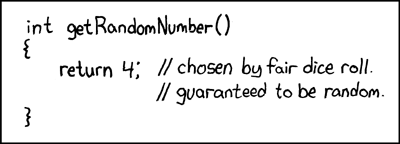
\includegraphics[width=2.5in,keepaspectratio]{random_number.png}
\end{center}
\bigskip \bigskip {\scriptsize Source:
  \url{http://imgs.xkcd.com/comics/random_number.png}, used under
  \url{http://www.xkcd.com/license.html}}
\end{frame}

\begin{frame}
  \frametitle{Actual Example Setup}
  Great, we will randomly set $\zeta = 4$ for all encryptions.
\end{frame}

\begin{frame}
  \frametitle{Example Query}
  \begin{itemize}
    \item Since $H(T_0) = 6$, 
      \begin{align*}
        \mathcal{E}_6 &= \mathcal{E}(2^{0\cdot2})\\
          &= 639
      \end{align*}
    \item Similarly, since $H(T_1) = 2$, 
      \begin{align*}
        \mathcal{E}_2 &= \mathcal{E}(2^{1\cdot2})\\
          &= 359.
      \end{align*}
    \item All other terms are encryptions of $0$; we will write these as $1$
      even though they would in fact be distributed across a wide array of
      values in \zmodntunits.
  \end{itemize}
\end{frame}


\begin{frame}
  \frametitle{Example Response}
  Suppose, as in our example above, that the responder inputs, in order, are
  $(T_0,D^0)$, $(T_1,D^1)$, $(5, D^2)$, and $(T_0,D^3)$, after
  which point the responder returns (perhaps another $T_0$ comes in, thus causing
  $c_{\mathcal{T}_0}$ to be greater than $r$). Here, 
  \begin{align*}
    D^0 &= 0000 = (D^0_0, D^0_1) = (00, 00),\\
    D^1 &= 0110 = (D^1_0, D^1_1) = (01, 10),\\
    D^2 &= 0111 = (D^2_0, D^2_1) = (01, 11),\\
    D^3 &= 0010 = (D^3_0, D^3_1) = (00, 10),\\
  \end{align*}~\\

  Note that since $5$ is not a search term, it will result in raising an
 encrypted zero to $D^2=7$; again, we're just going to write $1$, even though the
  acutal algorithm may (will) have any encryption of $0$ instead.
\end{frame}

\begin{frame}
  \frametitle{Example Response Matrix}
  The responder forms the matrix
  \begin{center}
  \begin{tabular}{c  C{2.25cm}  C{2.25cm}  C{2.25cm}  C{2.25cm}  }
     {\scriptsize Index}             & $\mathcal{Y}_0$ & $\mathcal{Y}_1$ & $\mathcal{Y}_2$ & $\mathcal{Y}_{3}$\\\toprule
     $\vdots$ & \multicolumn{4}{l}{$\qquad$}\\
     {\footnotesize{\tiny $2$}} & {\tiny $\mathcal{E}_2^{D^1_0}\mod N^2 = 359$} & {\tiny $\mathcal{E}_2^{D^1_1}\mod N^2 = 256$}      & 1                      & 1\\
     {\tiny $\vdots$} & \multicolumn{4}{l}{{\tiny $\qquad$}}\\
     {\footnotesize{\tiny $6$}}  & {\tiny $\mathcal{E}_6^{D^0_0} \mod N^2 = 1$} & {\tiny$\mathcal{E}_6^{D^0_1}\mod N^2 = 1$} & {\tiny $\mathcal{E}_6^{D^3_0}\mod N^2 = 1$}    &  {\tiny $\mathcal{E}_6^{D^3_1}\mod N^2 = 396$} \\   
     {\footnotesize{\tiny $7$}}  & 1 & 1 & 1                      & 1\\
     {\tiny $\vdots$} & \multicolumn{4}{l}{{\tiny $\qquad$}}\\\bottomrule
  \end{tabular}
  \end{center}
\end{frame}

\begin{frame}
  \frametitle{Example Responses}
  The only interesting responses are $\mathcal{Y}_0 = 359$, $\mathcal{Y}_1=256$, and $\mathcal{Y}_3 = 396$ (products are taken down columns).
\end{frame}

\begin{frame}
  \frametitle{Example Result}
  We decrypt to $Y_0=0100$, $Y_1 =8 = 1000 $ and $Y_3 = 2 = 0010$, and then run through the processing algorithm:
  \begin{itemize}
    \item Data For $T_0$: $M=0011$
      \begin{itemize}
        \item $X_1 = 0$: 
          \begin{itemize}
            \item $D_0 = (Y_0 \& 0011)/2^0 = 00$
            \item $D_1 = (Y_1 \& 0011)/2^0 = 00$
          \end{itemize} 
        \item $X_2 = 2$:
          \begin{itemize}
            \item $D_0 = (Y_2 \& 0011)/2^0 = 00$
            \item $D_1 = (Y_3 \& 0011)/2^0 = 10$
          \end{itemize}
      \end{itemize}
  \end{itemize}
\end{frame}

\begin{frame}
  \frametitle{Example Result}
  We decrypted to $Y_0 = 0100$, $Y_1 =8 = 1000 $ and $Y_3 = 2 = 0010$, and then run through the processing algorithm:
  \begin{itemize}
    \item Data For $T_1$: $M=1100$.
      \begin{itemize}
        \item $X_1 = 6$: 
          \begin{itemize}
            \item $D_0 = (Y_0 \& 1100)/2^2 = 01$
            \item $D_1 = (Y_1 \& 1100)/2^2 = 10$
          \end{itemize} 
        \item $X_2 = 0$:
          \begin{itemize}
            \item $D_0 = (Y_2 \& 1100)/2^2 = 00$
            \item $D_1 = (Y_3 \& 1100)/2^2 = 00$
          \end{itemize}
      \end{itemize}
  \end{itemize}
  These results are precisely the data the responder had.$^*$\\~\\
  {\tiny *: We cannot distinguish the fact that $X_2$ is a non-response
  from the possibility that $X_2$ represents an actual return of a datum $D=0$
from the responder. In practice, one must avoid using $D=0$ to eliminate this
ambiguity}
\end{frame}
\end{document} 
